\section{Platform Overview}
\label{sec:overviw}
\begin{figure*}[!htbp]
  \centering
     \subfloat[dashboard]{%
  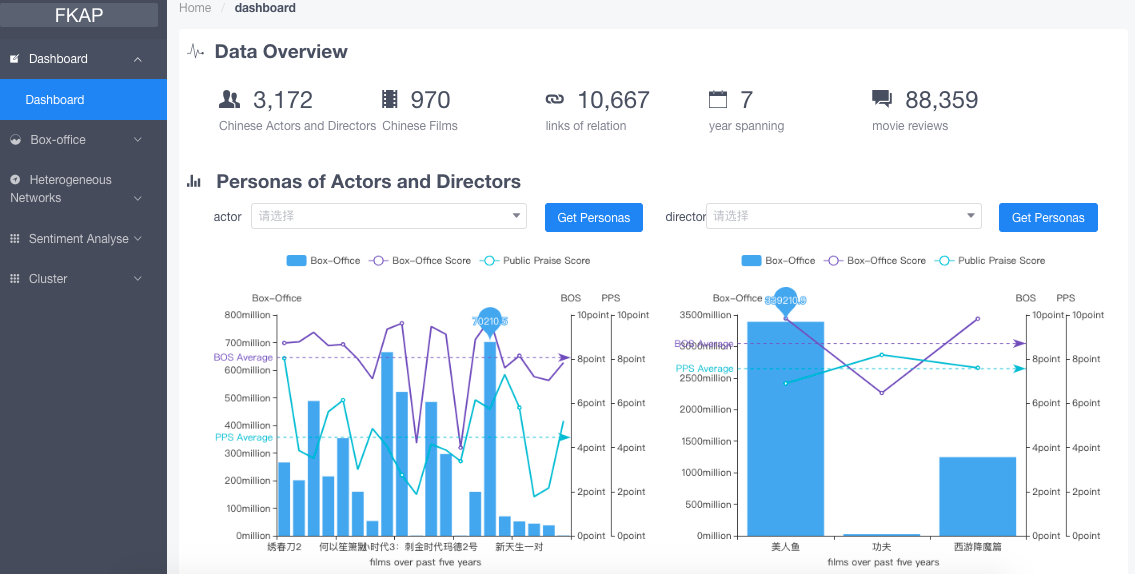
\includegraphics[width=2.0in]{screenshot5.png}}\hfill
    \subfloat[heterogeneous network]{%
  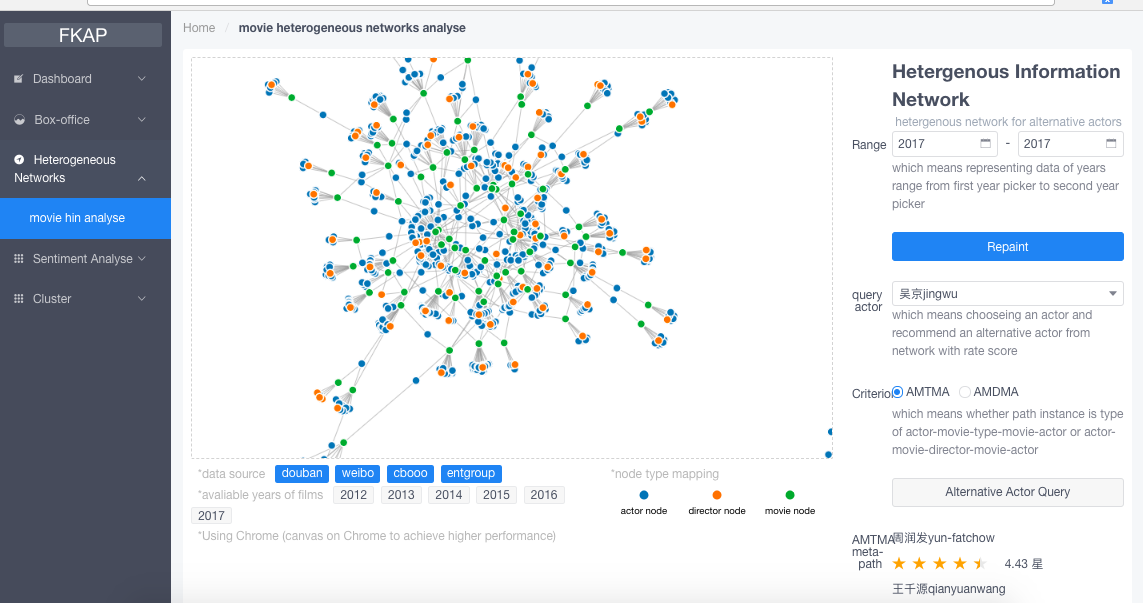
\includegraphics[width=2.0in]{screenshot1.png}}\hfill
    \subfloat[dynamic impact]{%
  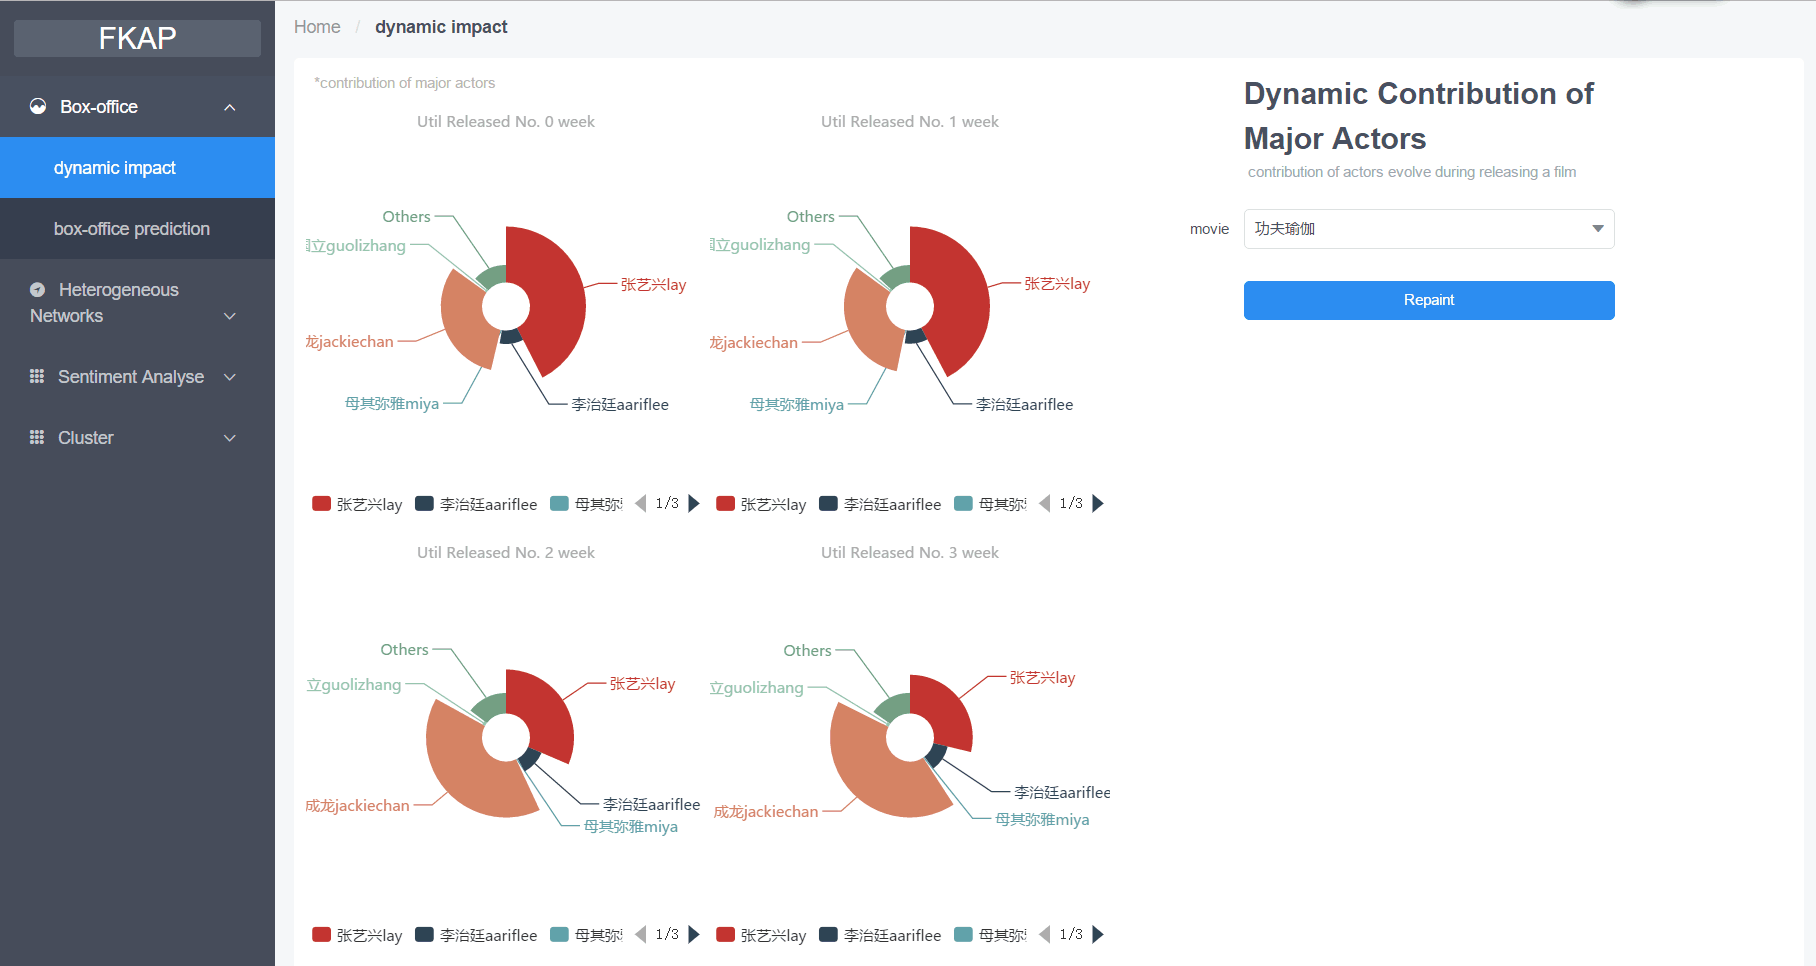
\includegraphics[width=2.0in]{screenshot2.png}}\hfill
    \subfloat[phased box-office predicting]{%
  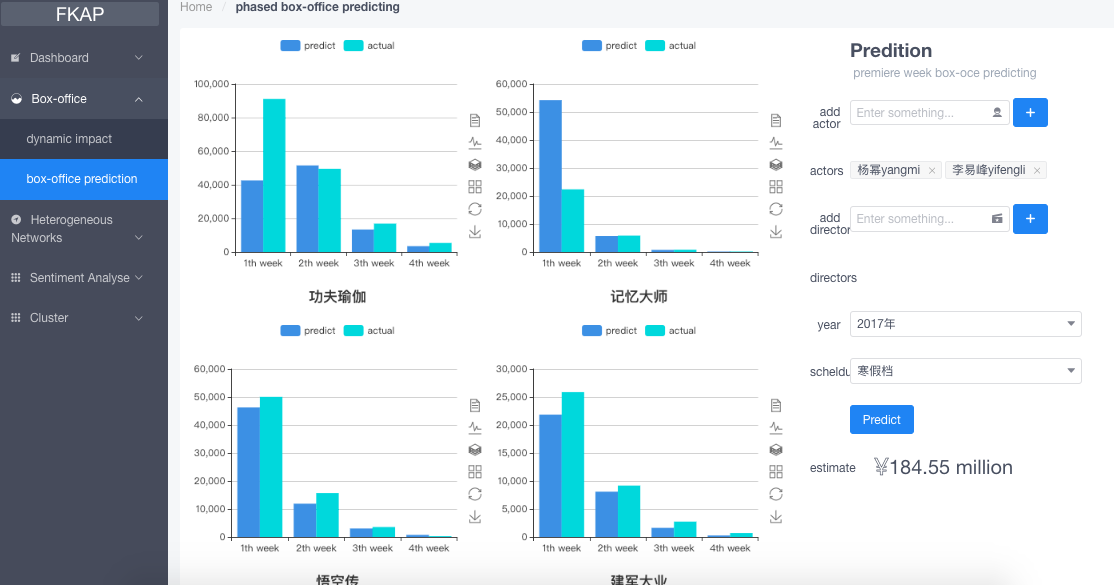
\includegraphics[width=2.0in]{screenshot3.png}}\hfill
%   \subfloat[film level sentiment]{%
%  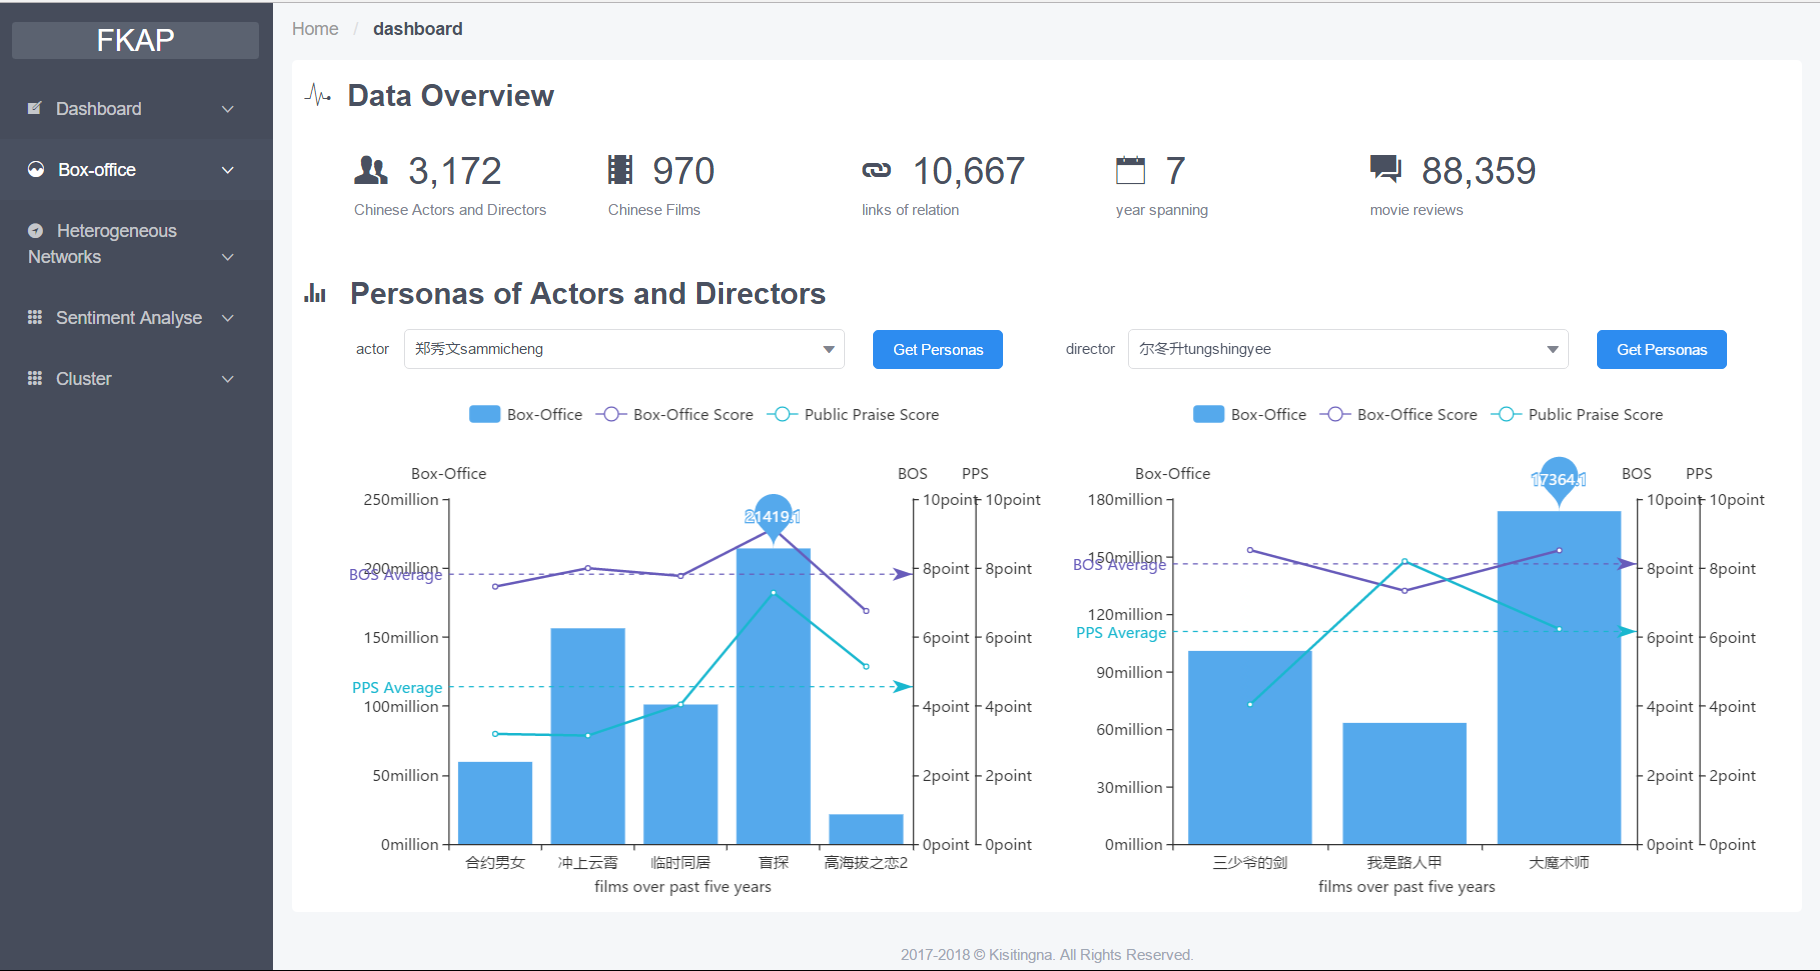
\includegraphics[width=2.0in]{screenshot4.png}}\hfill
 
  \caption{Screenshots of FKAP}
\end{figure*}

\begin{figure}[!htbp]
\centering
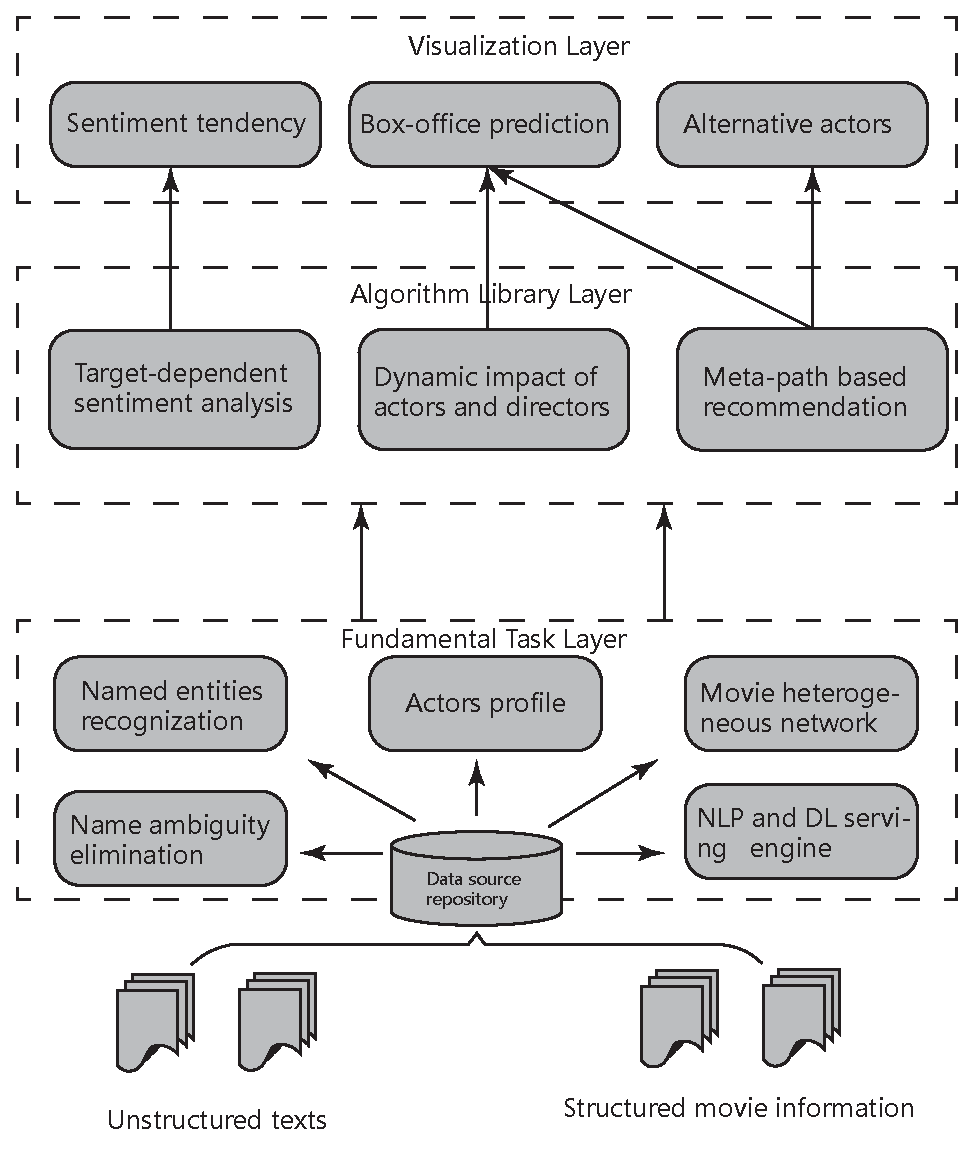
\includegraphics[width=0.8\columnwidth]{overview.eps}
\caption{System architecture}
\label{fig:mhin}
\end{figure}

\system is a web-based integrated system for movie analysis. The screenshots of \system are shown in Figure 1 and the architecture overview is displayed in Figure 2. Using \system, users can carry out a series of analysis based on the movie centric information.
\par In general, \system consists of three layers of components, including Basic Processing Task Layer, Higher Algorithm Library Layer and Visualization Layer.
\par Basic Processing Task Layers provides data cleaning, data standardization and data conversion. Due to the different data sources, the data obtained can not be applied directly to the analysis. In fact, the movie data need to consider the following questions, name ambiguity elimination, used to evaluate the quality of the film at the box office, the film's reviews of object identification, actor knowledge base construction. These methods are provided in the basic processing task layer.
\par Higer Algorithm Library Layer contains the core technology of \system, including Target-Dependent Sentiment Analysis Module and Dynamic Impact of Actors and Directors Module. The layer considers the importance of film reviews to a film and combine with Machine Learning.
\par Visualization Layer is the interface between the system and the users. To intuitively present the analysis results, this layer is designed to be user-friendly and easy to operate. Specifically, Sentiment Tendency is ... 